Agregando el controlador calculado anteriormente en el sistema se tiene el diagrama de bloques de la figura \ref{fig:diagrama de bloques con valores}.

\begin{figure}[h]
	\centering
	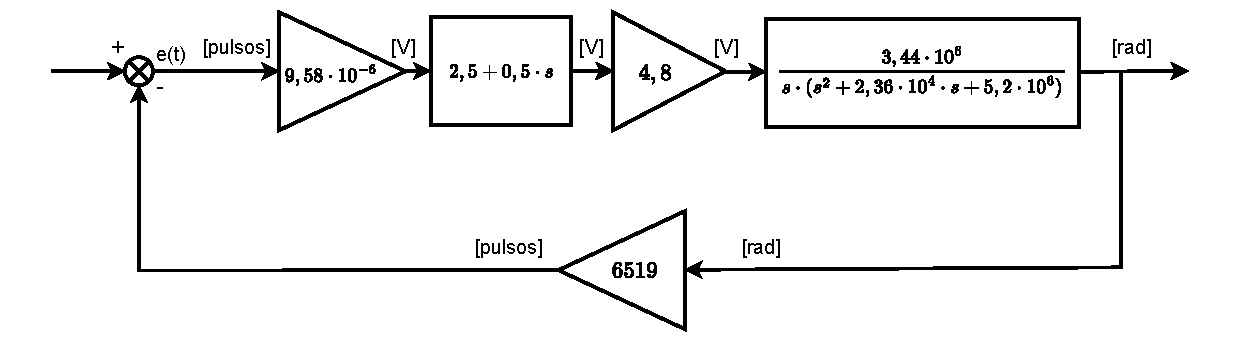
\includegraphics[width=1\textwidth]{img/diagrama_de_bloque_con_valores.pdf}
	\caption{Diagrama de bloques del sistema controlado con valores numéricos}
	\label{fig:diagrama de bloques con valores}
\end{figure}	

En la figura \ref{respuestacontrolada} se tiene la respuesta temporal del sistema lineal con el controlador ante un escalón de 521518 pulsos el cual representa un recorrido completo. 

Como se puede observar el sistema no presenta sobrepasamiento, error en estado estable y ademas el tiempo de asentamiento es de $8,5$  segundos, y llegando a un valor en estado estacionario de $\SI{80}{\radian}$, este valor esta relacionado con la distancia recorrida por la cortina de la siguiente manera:

\[
d = \theta \cdot r = \SI{80}{\radian} \cdot \SI{0,015}{\meter} = \SI{1,2}{\meter}
\]

Esto significa que el error en estado estable es cero, y ademas no se observa sobrepasamiento concluyendo que se cumplen las especificaciones de diseño establecidas.

\begin{figure}[h]
	\centering
	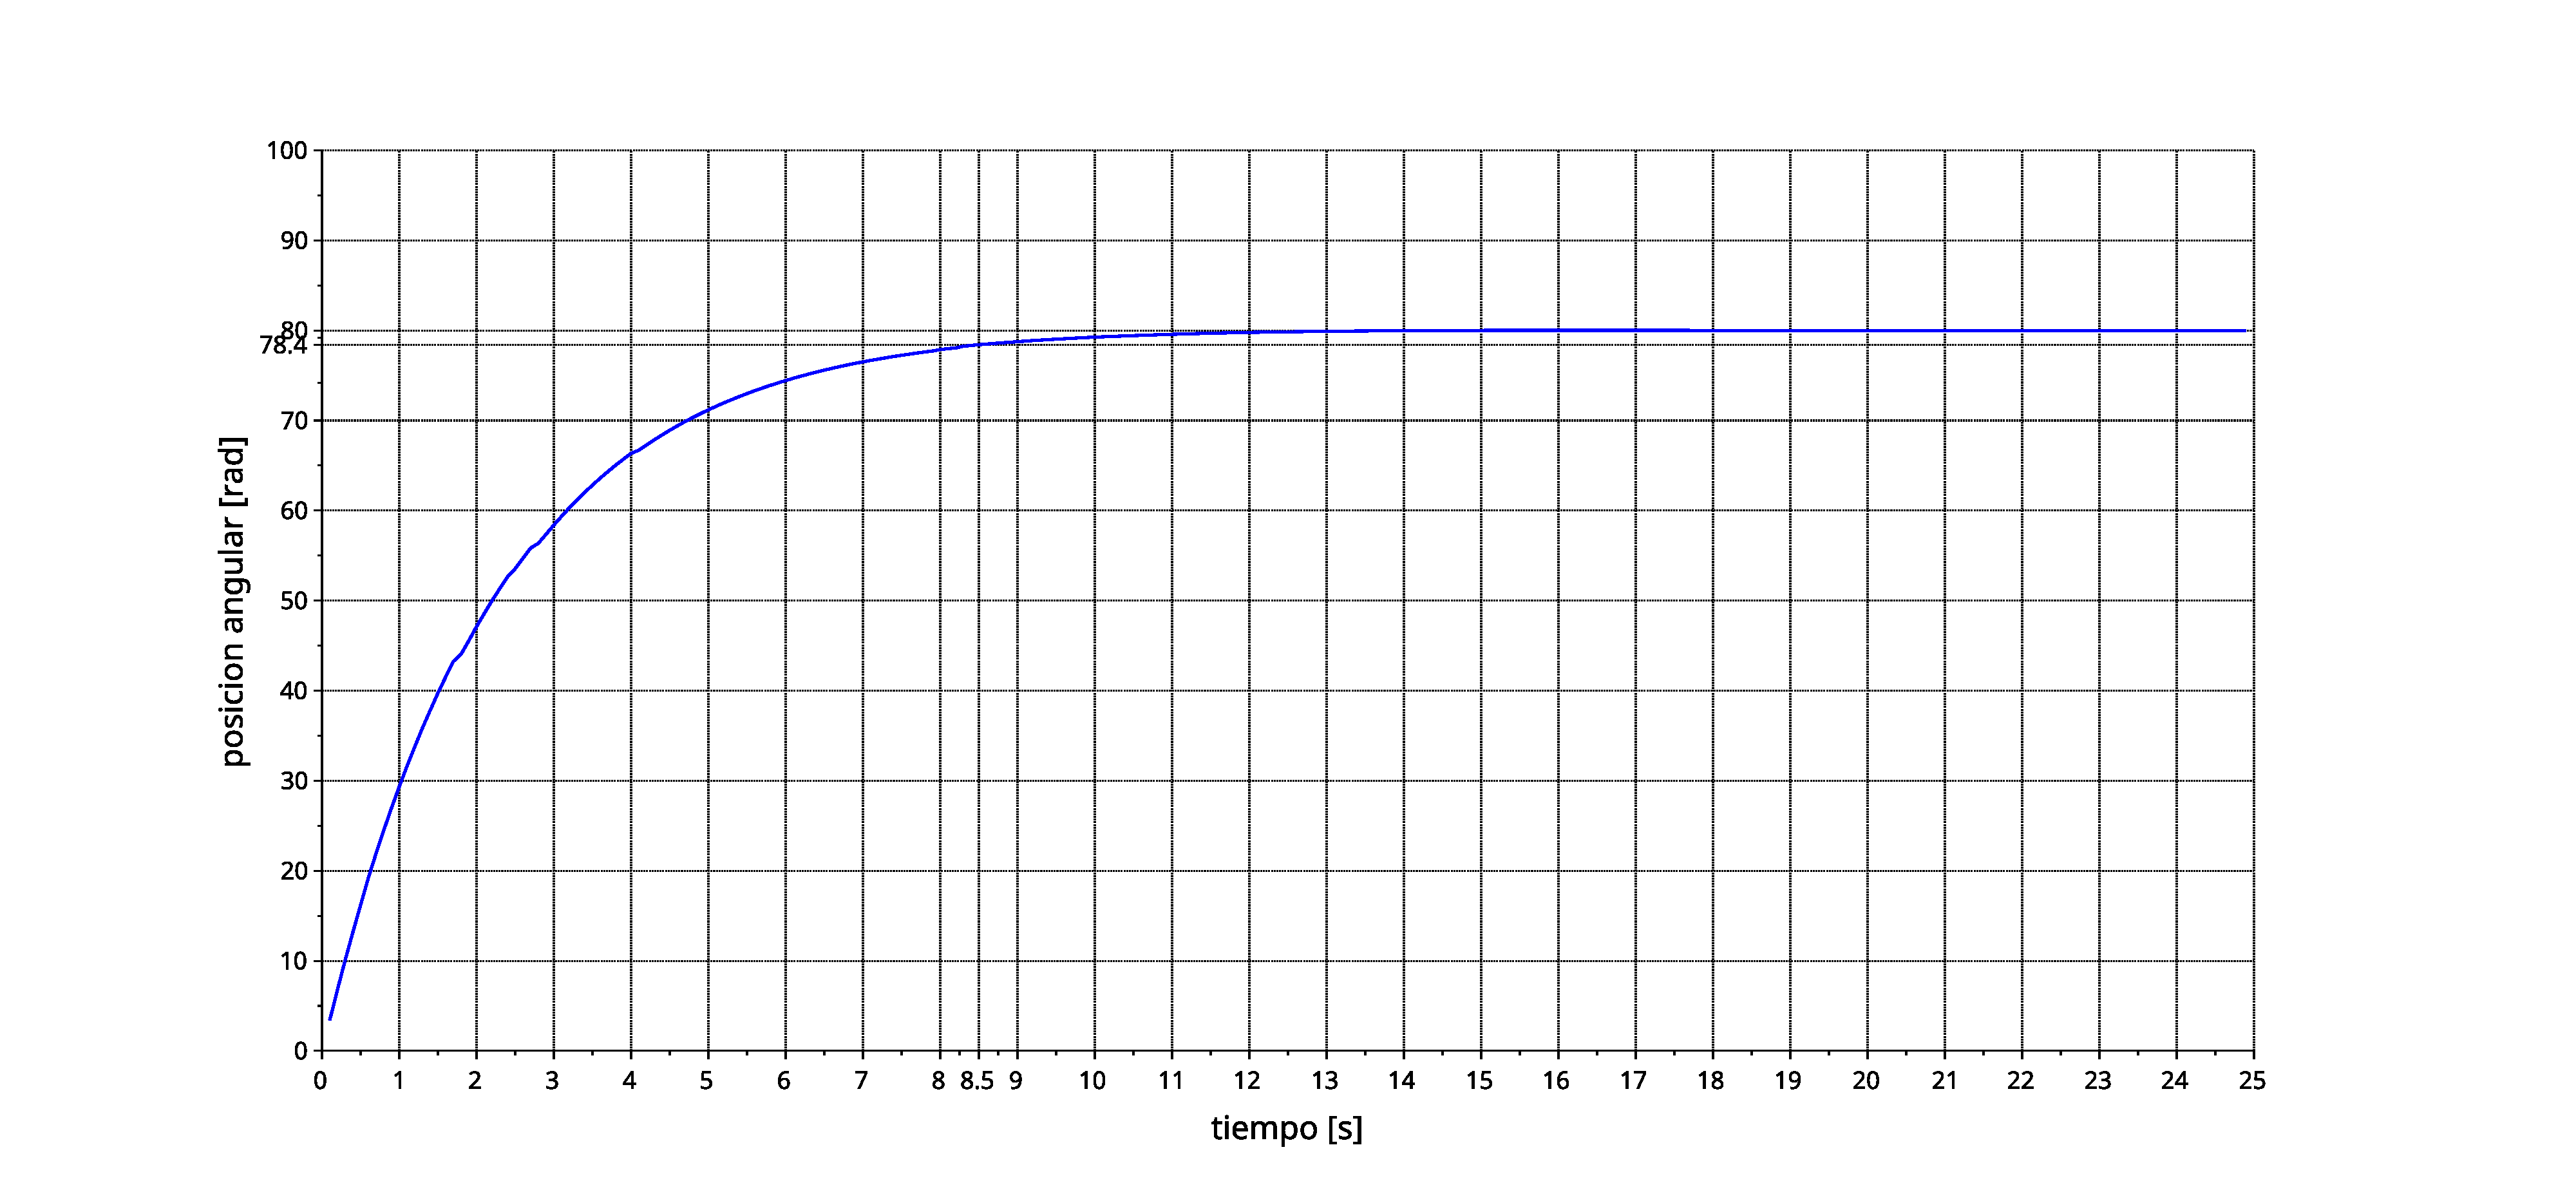
\includegraphics[width=1\textwidth]{img/respuesta_escalon_controlado.pdf}
	\caption{Respuesta temporal del sistema controlado a un escalón de amplitud 521518 pulsos}
	\label{respuestacontrolada}
	
\end{figure}

\newpage
\subsubsection{Simulación considerando no linealidades}

En la figura \ref{ddb_sim} se muestra el diagrama de bloques del sistema modelado utilizando el software \textit{Scilab} considerando las no linealidades mencionadas en la sección \ref{no_linealidades}, estas son:

\begin{itemize}
	\item Saturador: Limita la señal de control al rango de tensión disponible del motor, impidiendo que el controlador solicite valores mayores a la alimentación máxima. En este caso, restringe la acción de control al intervalo $\pm\SI{24}{V}$ que corresponde a la tensión nominal.
	
	\item Zona muerta (dead zone): Representa el margen de señal en el que el motor no genera movimiento debido a fricción interna y tolerancias mecánicas. Para valores de tensión dentro de este rango, la salida permanece nula, lo cual provoca un umbral mínimo necesario para iniciar el movimiento. El valor de tensión de zona muerta $\pm V_{dz}$ se calcula a partir de la corriente de arranque en vacío $I_o$ y la resistencia de armadura $R_a$ obtenidos de la hoja de datos:
	
	\[
	V_{dz} = I_o \cdot R_a = \SI{0,066}{\ampere} \cdot \SI{5,9}{\ohm} \approx \SI{0,39}{\volt}
	\]
	
Se optó por omitir el efecto de cuantización del sensor rotativo incremental. Si bien el encoder IE3-1024 transforma el desplazamiento angular continuo en pulsos discretos , el análisis de resolución lineal determinó que cada pulso representa un avance aproximado de solo $9,2 \cdot 10^{-5} \text{ m}$ ($0,09 \text{ mm}$). Dada la magnitud de este valor en comparación con el recorrido total de $1,2 \text{ m}$ , el error de redondeo intrínseco se consideró insignificante para la dinámica macroscópica del sistema.
\end{itemize}



\begin{figure}[h]
	\centering
	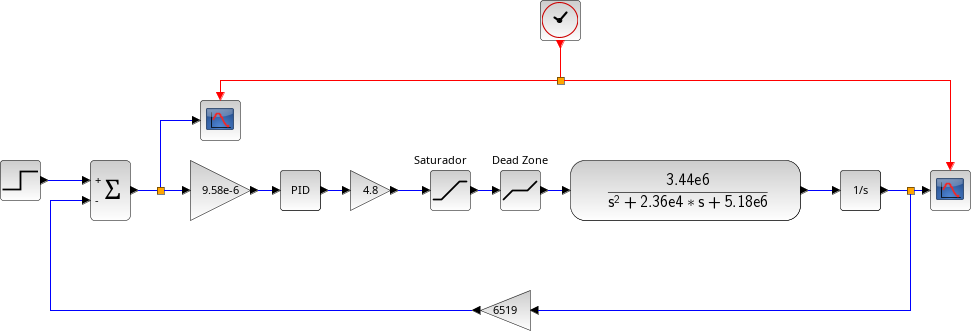
\includegraphics[width=1\textwidth]{img/diagrama_de_bloques_simulacion.png}
	\caption{Diagrama de bloques del sistema considerando no linealidades}
	\label{ddb_sim}
\end{figure}

Considerando las no linealidades antes mencionadas se realizó la simulación del sistema obteniendo la siguiente respuesta temporal ante una entrada tipo escalón de 521518 pulsos

\begin{figure}[h]
	\centering
	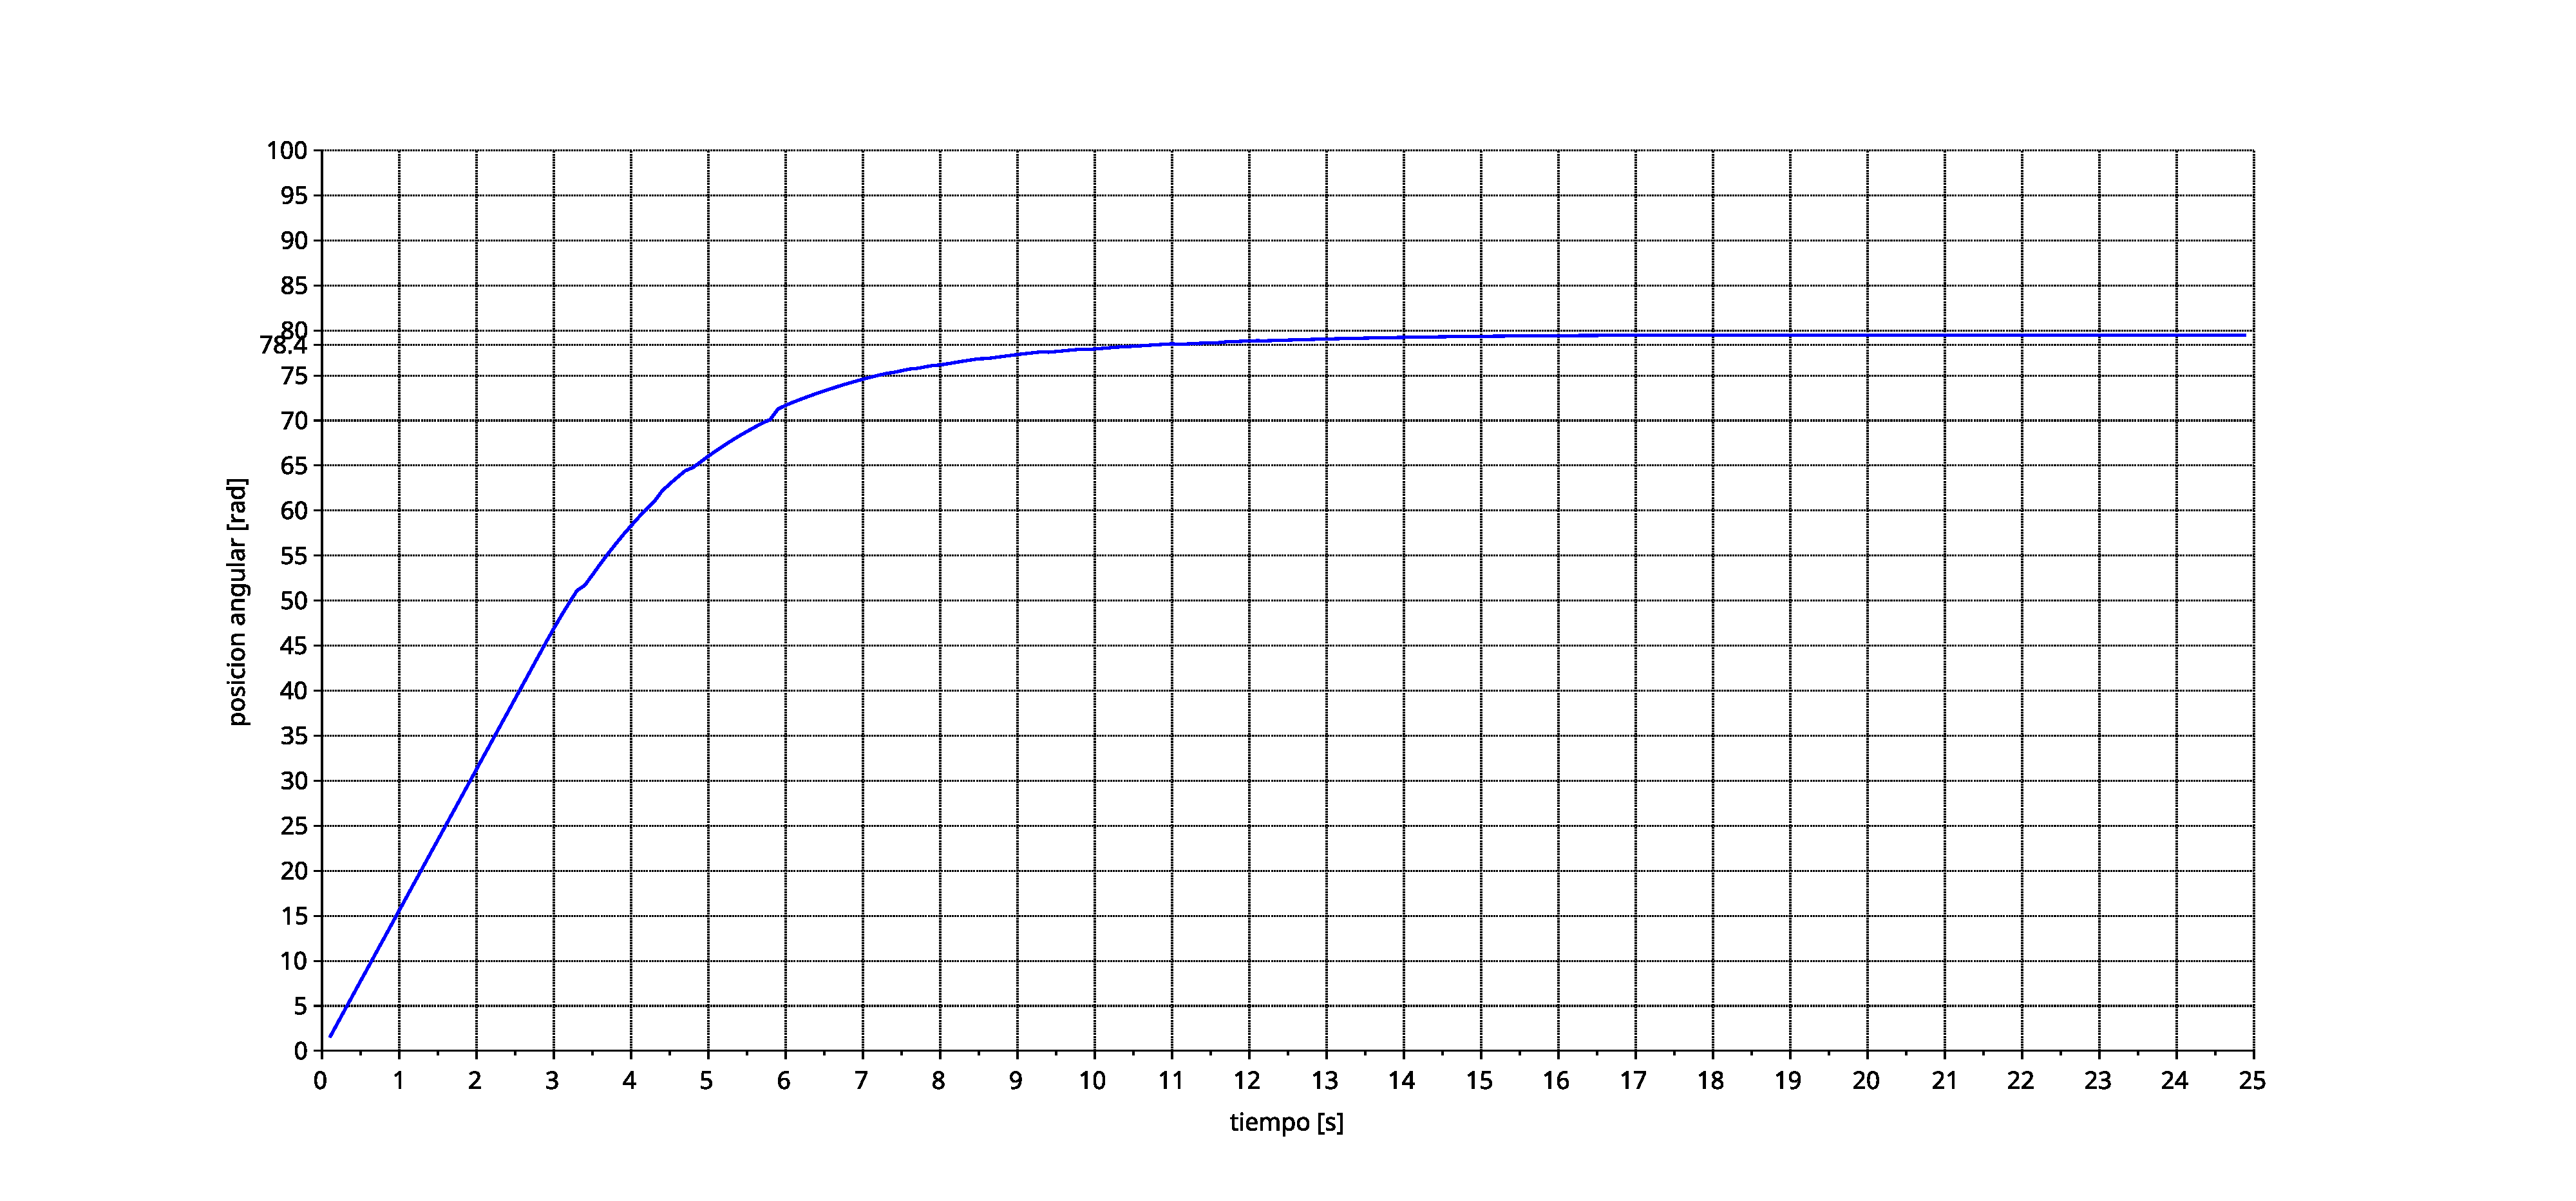
\includegraphics[width=1.1\textwidth]{img/simulacion_no_linealidades.pdf}
	\caption{Respuesta temporal considerando no linealidades ante una entrada tipo escalón de 521518 pulsos de amplitud}
	\label{respuesta_temporal_simulacion}
	
	\centering
	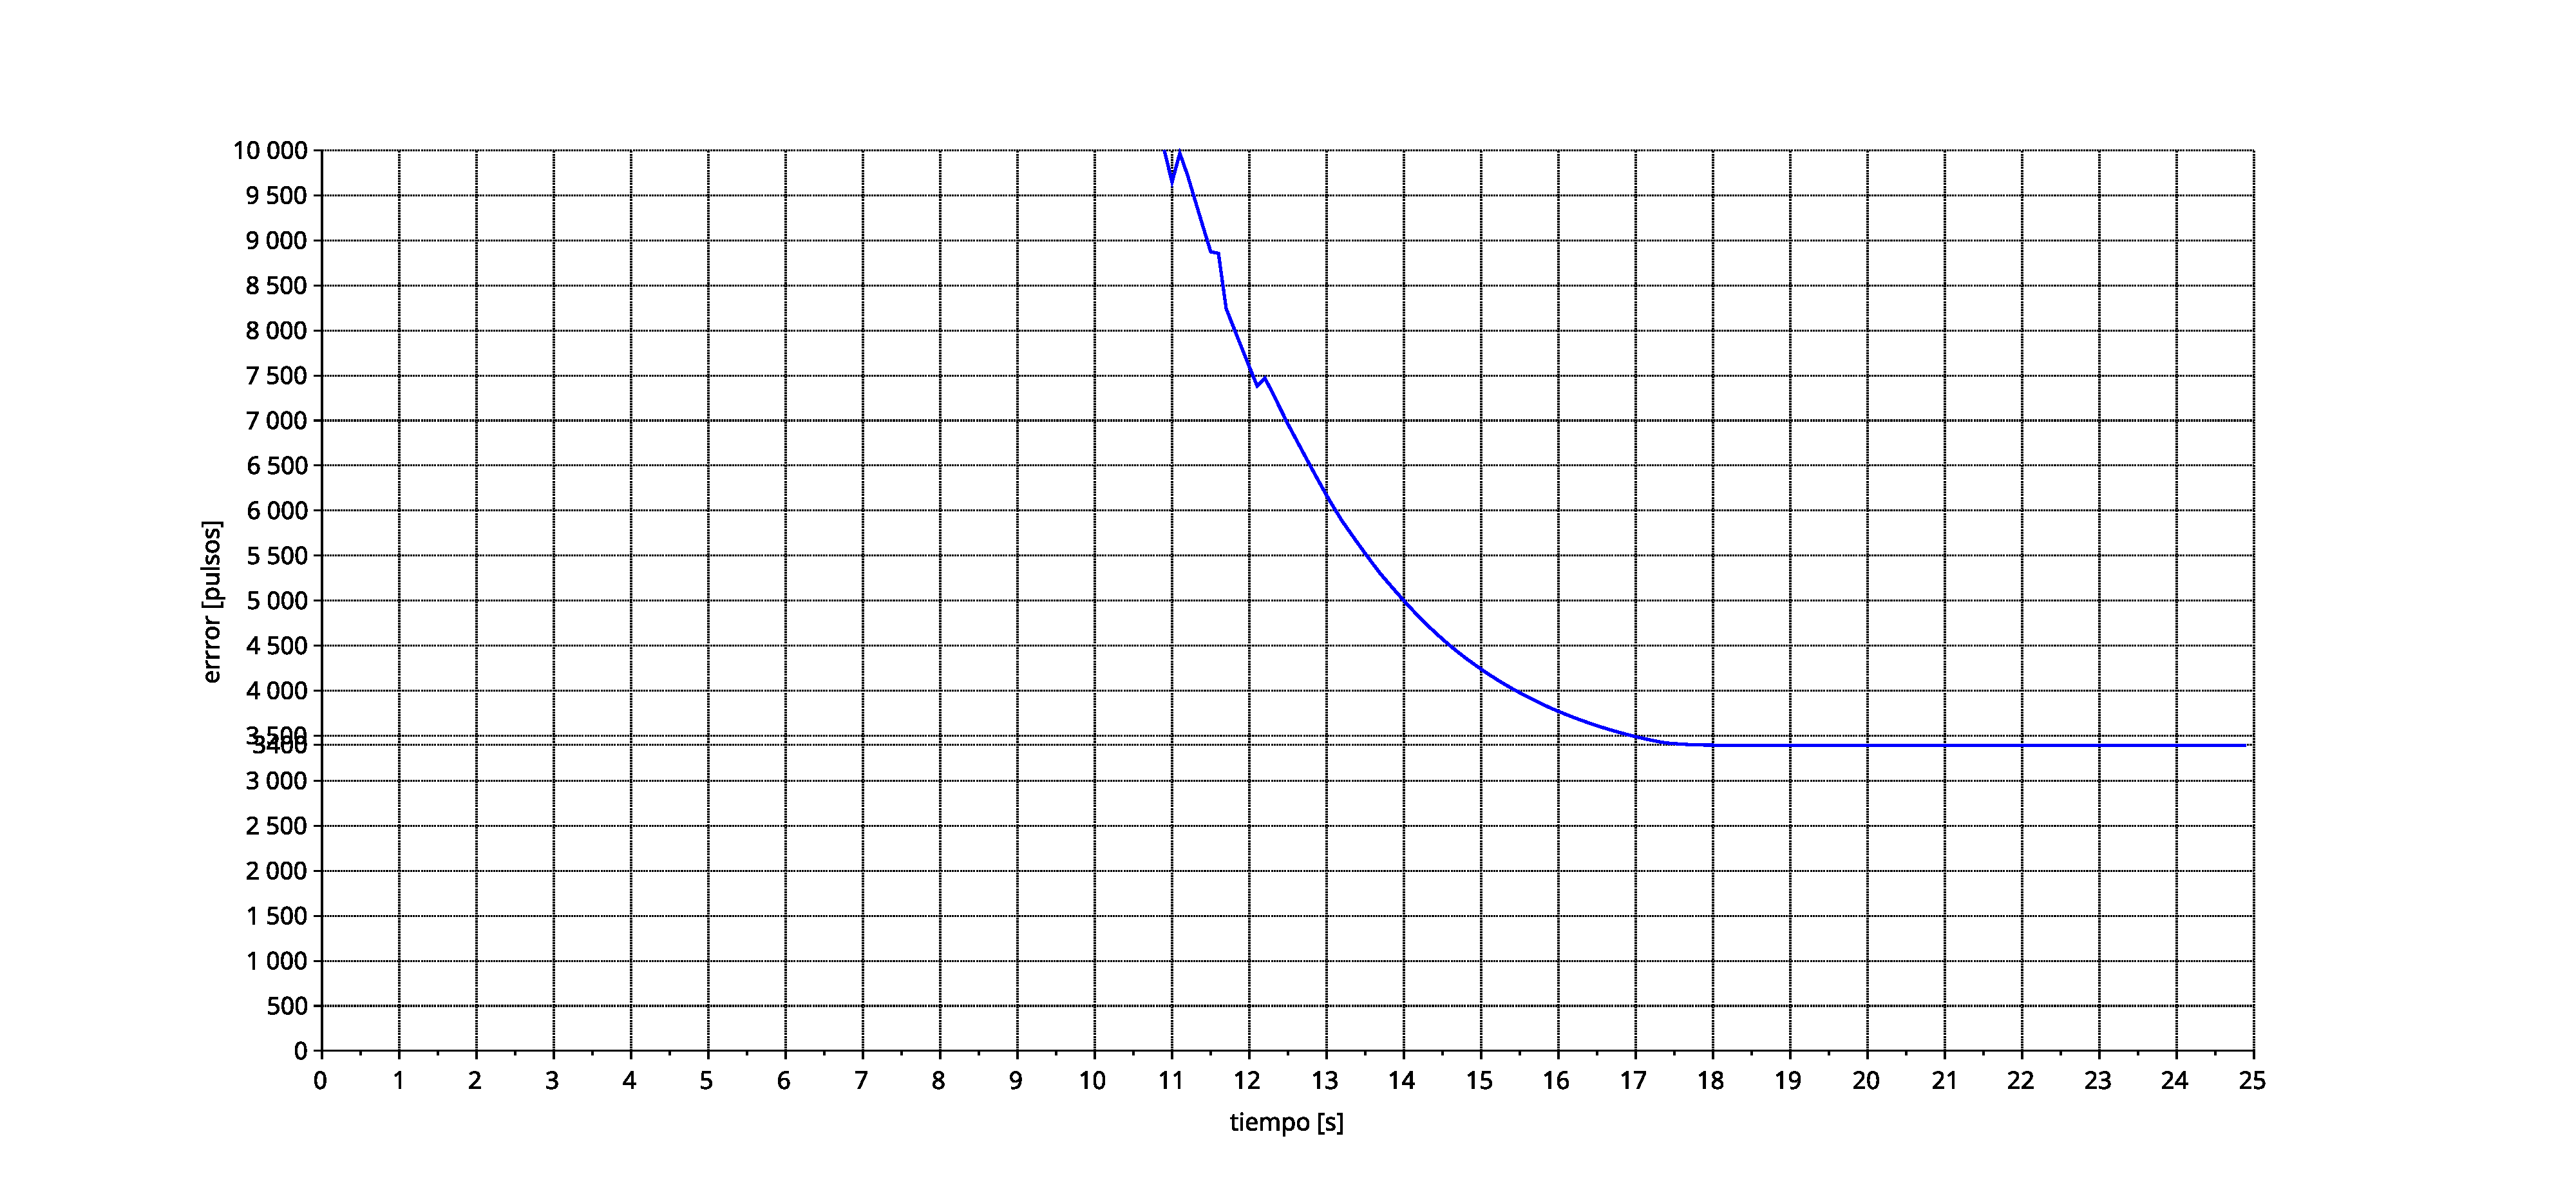
\includegraphics[width=1.1\textwidth]{img/simulacion_error.pdf}
	\caption{Señal de error considerando no linealidades ante una entrada tipo escalón de 521518 pulsos de amplitud}
	\label{error_sim}
\end{figure}

Como se observa en las figuras \ref{respuesta_temporal_simulacion} y \ref{error_sim}, la incorporación de las no linealidades aumenta el tiempo de establecimiento, pasando de 8,5 a 11 segundos, presenta error en estado estable de 3400 pulsos aproximadamente (lo que corresponde a $\SI{0,76}{\centi\meter}$) debido al efecto de la zona muerta y no se produce sobrepasamiento.
